\section{Functional Form Fits and Extrapolations}
\label{section:functional_form_fits}

We now show the fits and/or extrapolations of various functional forms. In all plots here and in the appendix, black points are the points used for fitting a functional form, green points are the held-out points used for evaluating extrapolation of a functional form fit to the black points, and a red line is the BNSL that has been fit to the black points.

In the tables and elsewhere, 
\begin{itemize}
    \item M1 refers to functional form $y = ax^b$
    \item M2 refers to functional form $y = ax^b +c$
    \item M3 refers to functional form $y = a(x^{-1} + d)^{-b} + c$
    \item M4 refers to functional form $(y - \epsilon_{\infty}) / ((\epsilon_{0} - y)^a) = bx$
\end{itemize}

All the extrapolation evaluations reported in the tables are reported in terms of root mean squared log error (RMSLE\footnote{RMSLE = $ \sqrt{(\sum_{i=1}^{n} (log(y_{i})-log(\hat{y}_{i}))^2)/n}$}) ± root standard log error. 

TODO: define root standard log error; see commented out lines for how it's calculated
\[error = (log(y_{i})-log(\hat{y}_{i}))^2)\] 
\[\mu_{error} = \frac{1}{N}\sum_{i=1}^N error\]
\[\sigma_{error} = \sqrt{\frac{1}{N-1}\sum_{i=1}^N(error_i-\mu_{error})^2}\]
\[rstderr = \sqrt{\mu_{error} + \frac{\sigma_{error}}{\sqrt{len(\hat{y})}}} - \sqrt{\mu_{error}}\] 
% how root standard log error is calculated
%error = (np.log(yp) - np.log(y)) ** 2
%errmu = np.mean(error)
%rstderr = np.sqrt(errmu + np.std(error) / (len(yp)**0.5)) - np.sqrt(errmu)

\FloatBarrier
\subsection{Vision}
\label{section:scaling_benchmark__vision}

(TODO: this sentence is repeated in language section)

Using the scaling laws benchmark of \cite{Alabdulmohsi2022revisiting}, we evaluate how well various functional forms extrapolate performance on vision tasks as training dataset size increases. In this vision subset of the benchmark, the tasks that are evaluated are error rate on each of various few-shot downstream image classification (IC) tasks; the downstream tasks are: Birds 200 \cite{welinder2010caltech}, Caltech101 \cite{fei2004learning}, CIFAR-100 \cite{krizhevsky2009learning}, and ImageNet \cite{deng2009imagenet}. The following architectures of various sizes are pretrained on subsets of JFT-300M: big-transfer residual neural networks (BiT) \cite{kolesnikov2020big}, MLP mixers (MiX) \cite{tolstikhin2021mlp}, and vision transformers (ViT) \cite{dosovitskiy2020image}. As can be seen in Table  \ref{table:scaling_laws_benchmark_dataset__Vision}, BNSL (TODO: make sure BNSL abbreviation is defined somewhere) yields extrapolations with the lowest RMSLE (Root Mean Squared Logarithmic Error) for the largest number (by a very large margin) (TODO: replace "large margin" with numbers) of tasks of any of the functional forms.

To view all plots of the BNSL on each of these tasks, see figures
\ref{fig:scaling_laws_benchmark_dataset__birds},
\ref{fig:scaling_laws_benchmark_dataset__cifar_100},
\ref{fig:scaling_laws_benchmark_dataset__caltech},
\ref{fig:scaling_laws_benchmark_dataset__ImageNet} in Appendix \ref{section:Plots_of_BNSL_Extrapolations}. To view all plots of M1, M2, M3, and M4 on each of these tasks, see Appendix A.4 of \cite{Alabdulmohsi2022revisiting}.

% \begin{center}
\begin{table}
    \centering
    \begin{tabular}{ |c|c|c|c|c|c|c| } 
\hline
Domain & \hspace{.9cm}Task & M1 $\uparrow$ & M2 $\uparrow$ & M3 $\uparrow$ & M4 $\uparrow$ & BNSL $\uparrow$ \\
 \hline
 IC & Birds 200 & 0 & 0 & 0 & 5.56 & \highlight{94.44}\\ 
 IC & Caltech101 & 0 & 0 & 5.56 & 5.56 & \highlight{88.89}\\ 
 IC & CIFAR-100 & 0 & 5.56 & 5.56 & 5.56 & \highlight{83.33}\\
 IC & ImageNet & 0 & 0 & 11.11 & 0 & \highlight{88.89}\\
 Language & All & 5 & 10 & 15 & 25 & \highlight{45}\\
 \hline
\end{tabular}
    \caption{
    Percentage of tasks by domain where each functional form is the best for extrapolation. See Section \ref{section:scaling_benchmark__vision} for more details. Numbers for M1, M2, M3, and M4 were obtained via correspondence with authors of \cite{Alabdulmohsi2022revisiting}. 
    }
    \label{table:scaling_laws_benchmark_dataset__Vision}
\end{table}
% \end{center}

\begin{table}[htbp]
\tiny
% \fontsize{8}{8}\selectfont
% \setlength\tabcolsep{3.1pt} 
\begin{tabular}
%{p{.02\textwidth}p{.165\textwidth}p{.095\textwidth}p{.01\textwidth}p{.01\textwidth}p{.099\textwidth}p{.099\textwidth}p{.099\textwidth}p{.099\textwidth}p{.099\textwidth}}
{p{.205\textwidth}p{.111\textwidth}p{.099\textwidth}p{.099\textwidth}p{.099\textwidth}p{.099\textwidth}p{.099\textwidth}}
%\begin{tabular}{llllrrrrrrrrrrrrl}
\hspace{.9cm}Task & Model & M1 $\downarrow$ & M2 $\downarrow$ & M3 $\downarrow$ & M4 $\downarrow$ & BNSL $\downarrow$ \\
\hline
Birds 200 10-shot & BiT/101/3 & 9.13e-2 & 9.13e-2 & 9.13e-2 & 2.49e-2 & \highlight{3.79e-3} \\
Birds 200 10-shot & BiT/50/1 & 6.88e-2 & 6.88e-2 & 5.24e-2 & 2.48e-2 & \highlight{4.96e-3} \\
Birds 200 10-shot & MiX/B/16 & 9.15e-2 & 9.15e-2 & 3.95e-2 & 4.14e-2 & \highlight{9.98e-3} \\
Birds 200 10-shot & MiX/L/16 & 5.51e-2 & 5.51e-2 & 5.51e-2 & 4.59e-2 & \highlight{8.41e-3} \\
Birds 200 10-shot & ViT/B/16 & 6.77e-2 & 6.77e-2 & 3.52e-2 & 1.87e-2 & \highlight{9.81e-3} \\
Birds 200 10-shot & ViT/S/16 & 3.95e-2 & 3.95e-2 & 3.74e-2 & \highlight{9.81e-3} & 1.51e-2 \\
Birds 200 25-shot & BiT/101/3 & 9.41e-2 & 9.41e-2 & 9.41e-2 & 5.09e-2 & \highlight{7.24e-3} \\
Birds 200 25-shot & BiT/50/1 & 1.10e-1 & 7.29e-2 & 1.52e-2 & 1.63e-2 & \highlight{8.00e-3} \\
Birds 200 25-shot & MiX/B/16 & 1.40e-1 & 1.40e-1 & 6.93e-2 & 1.85e-2 & \highlight{5.02e-3} \\
Birds 200 25-shot & MiX/L/16 & 1.12e-1 & 1.12e-1 & 1.12e-1 & 4.88e-2 & \highlight{1.05e-2} \\
Birds 200 25-shot & ViT/B/16 & 9.02e-2 & 9.02e-2 & 3.75e-2 & 1.52e-2 & \highlight{5.87e-3} \\
Birds 200 25-shot & ViT/S/16 & 5.06e-2 & 5.06e-2 & 4.96e-2 & 3.28e-2 & \highlight{1.21e-2} \\
Birds 200 5-shot & BiT/101/3 & 8.17e-2 & 8.17e-2 & 8.17e-2 & 3.00e-2 & \highlight{6.08e-3} \\
Birds 200 5-shot & BiT/50/1 & 5.44e-2 & 5.44e-2 & 5.44e-2 & 2.63e-2 & \highlight{5.79e-3} \\
Birds 200 5-shot & MiX/B/16 & 8.27e-2 & 8.27e-2 & 5.49e-2 & 1.86e-2 & \highlight{5.74e-3} \\
Birds 200 5-shot & MiX/L/16 & 5.68e-2 & 5.68e-2 & 5.68e-2 & 2.65e-2 & \highlight{5.06e-3} \\
Birds 200 5-shot & ViT/B/16 & 3.40e-2 & 3.40e-2 & 3.40e-2 & 1.26e-2 & \highlight{6.32e-3} \\
Birds 200 5-shot & ViT/S/16 & 2.75e-2 & 2.75e-2 & 2.75e-2 & 1.56e-2 & \highlight{6.93e-3} \\
\hline
CIFAR-100 10-shot & BiT/101/3 & 8.57e-2 & 8.57e-2 & 8.25e-2 & 9.28e-2 & \highlight{1.53e-2} \\
CIFAR-100 10-shot & BiT/50/1 & 7.44e-2 & 1.24e-2 & 2.08e-2 & 1.23e-2 & \highlight{9.74e-3} \\
CIFAR-100 10-shot & MiX/B/16 & 8.77e-2 & 8.77e-2 & 2.71e-2 & 2.60e-2 & \highlight{8.61e-3} \\
CIFAR-100 10-shot & MiX/L/16 & 1.05e-1 & 1.05e-1 & 4.85e-2 & 4.76e-2 & \highlight{1.55e-2} \\
CIFAR-100 10-shot & ViT/B/16 & 8.98e-2 & 8.98e-2 & 8.98e-2 & 5.60e-2 & \highlight{1.73e-2} \\
CIFAR-100 10-shot & ViT/S/16 & 6.84e-2 & 2.11e-2 & 3.35e-2 & 2.47e-2 & \highlight{1.15e-2} \\
CIFAR-100 25-shot & BiT/101/3 & 8.77e-2 & 8.77e-2 & 4.44e-2 & 4.29e-2 & \highlight{9.32e-3} \\
CIFAR-100 25-shot & BiT/50/1 & 7.31e-2 & 2.35e-2 & 3.65e-2 & 2.36e-2 & \highlight{2.00e-2} \\
CIFAR-100 25-shot & MiX/B/16 & 1.08e-1 & 4.75e-2 & 2.10e-2 & 2.08e-2 & \highlight{8.15e-3} \\
CIFAR-100 25-shot & MiX/L/16 & 9.79e-2 & 9.79e-2 & 3.67e-2 & 2.79e-2 & \highlight{8.47e-3} \\
CIFAR-100 25-shot & ViT/B/16 & 1.07e-1 & 1.07e-1 & 6.54e-2 & \highlight{4.81e-2} & 1.20e-1 \\
CIFAR-100 25-shot & ViT/S/16 & 8.03e-2 & 2.19e-2 & 3.13e-2 & 2.19e-2 & \highlight{1.34e-2} \\
CIFAR-100 5-shot & BiT/101/3 & 5.94e-2 & 5.94e-2 & 5.94e-2 & 4.57e-2 & \highlight{1.58e-2} \\
CIFAR-100 5-shot & BiT/50/1 & 4.87e-2 & 4.87e-2 & \highlight{1.69e-2} & 4.91e-2 & 1.95e-2 \\
CIFAR-100 5-shot & MiX/B/16 & 7.07e-2 & 7.07e-2 & 2.78e-2 & 2.05e-2 & \highlight{6.77e-3} \\
CIFAR-100 5-shot & MiX/L/16 & 7.06e-2 & 7.06e-2 & 4.17e-2 & 3.14e-2 & \highlight{1.18e-2} \\
CIFAR-100 5-shot & ViT/B/16 & 6.27e-2 & 6.27e-2 & 6.27e-2 & 5.11e-2 & \highlight{1.19e-2} \\
CIFAR-100 5-shot & ViT/S/16 & 6.93e-2 & \highlight{2.84e-2} & 3.88e-2 & 3.09e-2 & 6.40e-2 \\
\hline
Caltech101 10-shot & BiT/101/3 & 3.07e-1 & 3.07e-1 & 1.51e-1 & 3.54e-2 & \highlight{6.42e-3} \\
Caltech101 10-shot & BiT/50/1 & 3.29e-1 & 7.68e-2 & 1.13e-1 & 6.31e-2 & \highlight{5.37e-3} \\
Caltech101 10-shot & MiX/B/16 & 1.35e-1 & 1.35e-1 & 1.35e-1 & 2.11e-1 & \highlight{3.72e-2} \\
Caltech101 10-shot & MiX/L/16 & 1.25e-1 & 1.25e-1 & 1.25e-1 & 1.92e-1 & \highlight{3.73e-2} \\
Caltech101 10-shot & ViT/B/16 & 7.76e-2 & 7.76e-2 & 3.11e-2 & 5.54e-2 & \highlight{1.67e-2} \\
Caltech101 10-shot & ViT/S/16 & 1.95e-1 & 3.41e-2 & \highlight{2.40e-2} & 3.95e-2 & 3.31e-2 \\
Caltech101 25-shot & BiT/101/3 & 1.15e-1 & 1.15e-1 & 1.15e-1 & 5.23e-2 & \highlight{1.13e-2} \\
Caltech101 25-shot & BiT/50/1 & 3.60e-1 & 8.80e-2 & 1.43e-1 & 5.95e-2 & \highlight{2.13e-3} \\
Caltech101 25-shot & MiX/B/16 & 8.28e-2 & 8.28e-2 & 8.28e-2 & 1.74e-1 & \highlight{2.83e-2} \\
Caltech101 25-shot & MiX/L/16 & 9.66e-2 & 9.66e-2 & 9.66e-2 & 1.03e-1 & \highlight{1.98e-2} \\
Caltech101 25-shot & ViT/B/16 & 1.03e-1 & 3.33e-2 & 4.46e-2 & 4.24e-2 & \highlight{6.37e-3} \\
Caltech101 25-shot & ViT/S/16 & 1.77e-1 & 3.79e-2 & 2.80e-2 & \highlight{2.35e-2} & 2.38e-2 \\
Caltech101 5-shot & BiT/101/3 & 2.12e-1 & 2.12e-1 & 2.12e-1 & 8.82e-2 & \highlight{3.17e-3} \\
Caltech101 5-shot & BiT/50/1 & 2.34e-1 & 4.13e-2 & 1.61e-2 & 4.49e-2 & \highlight{1.33e-2} \\
Caltech101 5-shot & MiX/B/16 & 2.43e-1 & 2.43e-1 & 2.35e-1 & 1.23e-1 & \highlight{3.59e-3} \\
Caltech101 5-shot & MiX/L/16 & 1.38e-1 & 1.38e-1 & 1.38e-1 & 3.19e-2 & \highlight{3.19e-2} \\
Caltech101 5-shot & ViT/B/16 & 1.10e-1 & 1.10e-1 & 6.02e-2 & 6.59e-2 & \highlight{2.33e-2} \\
Caltech101 5-shot & ViT/S/16 & 1.90e-1 & 3.82e-2 & 5.04e-2 & 4.06e-2 & \highlight{2.47e-2} \\
\hline
ImageNet 10-shot & BiT/101/3 & 1.27e-1 & 1.27e-1 & 7.36e-2 & 2.13e-2 & \highlight{5.95e-3} \\
ImageNet 10-shot & BiT/50/1 & 9.54e-2 & 9.54e-2 & \highlight{5.75e-3} & 1.77e-2 & 8.93e-3 \\
ImageNet 10-shot & MiX/B/16 & 9.34e-2 & 9.34e-2 & 3.37e-2 & 1.80e-2 & \highlight{5.88e-3} \\
ImageNet 10-shot & MiX/L/16 & 9.83e-2 & 9.83e-2 & 9.83e-2 & 9.48e-3 & \highlight{3.81e-3} \\
ImageNet 10-shot & ViT/B/16 & 4.62e-2 & 4.62e-2 & 4.62e-2 & 3.43e-2 & \highlight{2.85e-3} \\
ImageNet 10-shot & ViT/S/16 & 4.74e-2 & 4.74e-2 & 1.66e-2 & 1.14e-2 & \highlight{1.97e-3} \\
ImageNet 25-shot & BiT/101/3 & 1.42e-1 & 1.42e-1 & 6.67e-2 & 2.18e-2 & \highlight{4.86e-3} \\
ImageNet 25-shot & BiT/50/1 & 1.17e-1 & 1.17e-1 & \highlight{4.06e-3} & 1.70e-2 & 8.14e-3 \\
ImageNet 25-shot & MiX/B/16 & 9.59e-2 & 9.59e-2 & 5.39e-2 & 1.47e-2 & \highlight{2.86e-3} \\
ImageNet 25-shot & MiX/L/16 & 1.03e-1 & 1.03e-1 & 1.03e-1 & 6.09e-3 & \highlight{1.94e-3} \\
ImageNet 25-shot & ViT/B/16 & 5.17e-2 & 5.17e-2 & 5.17e-2 & 3.26e-2 & \highlight{6.91e-3} \\
ImageNet 25-shot & ViT/S/16 & 5.52e-2 & 4.12e-2 & 9.65e-3 & 1.16e-2 & \highlight{3.09e-3} \\
ImageNet 5-shot & BiT/101/3 & 9.24e-2 & 9.24e-2 & 9.24e-2 & 1.01e-2 & \highlight{2.55e-3} \\
ImageNet 5-shot & BiT/50/1 & 8.95e-2 & 8.95e-2 & 1.53e-2 & 1.03e-2 & \highlight{4.00e-3} \\
ImageNet 5-shot & MiX/B/16 & 9.09e-2 & 9.09e-2 & 3.01e-2 & 1.45e-2 & \highlight{3.57e-3} \\
ImageNet 5-shot & MiX/L/16 & 7.99e-2 & 7.99e-2 & 7.99e-2 & 5.66e-3 & \highlight{1.63e-3} \\
ImageNet 5-shot & ViT/B/16 & 4.11e-2 & 4.11e-2 & 4.11e-2 & 2.88e-2 & \highlight{4.97e-3} \\
ImageNet 5-shot & ViT/S/16 & 4.20e-2 & 4.20e-2 & 2.40e-2 & 1.44e-2 & \highlight{3.00e-3} \\
\end{tabular}
    \caption{
    Extrapolation Results for Vision Tasks. See Section \ref{section:scaling_benchmark__vision} for more details. Numbers for M1, M2, M3, and M4 obtained via correspondence with authors of \cite{Alabdulmohsi2022revisiting}. 
    }
    \label{table:scaling_laws_benchmark_dataset__Vision}
\end{table}
\FloatBarrier

\begin{table}[htbp]
\begin{adjustwidth}{-2.2cm}{-1cm}
\fontsize{8}{10}\selectfont
% \setlength\tabcolsep{3.1pt} 
\begin{tabular}
{|p{.165\textwidth} c c c c c || p{.165\textwidth} c c c c c |}
%{p{.02\textwidth}p{.165\textwidth}p{.095\textwidth}p{.01\textwidth}p{.01\textwidth}p{.099\textwidth}p{.099\textwidth}p{.099\textwidth}p{.099\textwidth}p{.099\textwidth}}
% {p{.165\textwidth}p{.070\textwidth}p{.070\textwidth}p{.080\textwidth}p{.080\textwidth}p{.080\textwidth}p{.165\textwidth}p{.080\textwidth}p{.080\textwidth}p{.080\textwidth}p{.080\textwidth}p{.080\textwidth}}
%\begin{tabular}{llllrrrrrrrrrrrrl}
\hline
\hspace{.9cm}Task & M1 $\downarrow$ & M2 $\downarrow$ & M3 $\downarrow$ & M4 $\downarrow$ & BNSL $\downarrow$ & \hspace{.9cm}Task & M1 $\downarrow$ & M2 $\downarrow$ & M3 $\downarrow$ & M4 $\downarrow$ & BNSL $\downarrow$\\
\hline
Birds 200 10-shot & 9.13e-2 & 9.13e-2 & 9.13e-2 & 2.49e-2 & \highlight{3.79e-3} & CIFAR-100 10-shot & 8.57e-2 & 8.57e-2 & 8.25e-2 & 9.28e-2 & \highlight{1.53e-2} \\
Birds 200 10-shot & 6.88e-2 & 6.88e-2 & 5.24e-2 & 2.48e-2 & \highlight{4.96e-3} & CIFAR-100 10-shot & 7.44e-2 & 1.24e-2 & 2.08e-2 & 1.23e-2 & \highlight{9.74e-3} \\
Birds 200 10-shot & 9.15e-2 & 9.15e-2 & 3.95e-2 & 4.14e-2 & \highlight{9.98e-3} & CIFAR-100 10-shot & 8.77e-2 & 8.77e-2 & 2.71e-2 & 2.60e-2 & \highlight{8.61e-3} \\
Birds 200 10-shot & 5.51e-2 & 5.51e-2 & 5.51e-2 & 4.59e-2 & \highlight{8.41e-3} & CIFAR-100 10-shot & 1.05e-1 & 1.05e-1 & 4.85e-2 & 4.76e-2 & \highlight{1.55e-2} \\
Birds 200 10-shot & 6.77e-2 & 6.77e-2 & 3.52e-2 & 1.87e-2 & \highlight{9.81e-3} & CIFAR-100 10-shot & 8.98e-2 & 8.98e-2 & 8.98e-2 & 5.60e-2 & \highlight{1.73e-2} \\
Birds 200 10-shot & 3.95e-2 & 3.95e-2 & 3.74e-2 & \highlight{9.81e-3} & 1.51e-2 & CIFAR-100 10-shot & 6.84e-2 & 2.11e-2 & 3.35e-2 & 2.47e-2 & \highlight{1.15e-2} \\
Birds 200 25-shot & 9.41e-2 & 9.41e-2 & 9.41e-2 & 5.09e-2 & \highlight{7.24e-3} & CIFAR-100 25-shot & 8.77e-2 & 8.77e-2 & 4.44e-2 & 4.29e-2 & \highlight{9.32e-3} \\
Birds 200 25-shot & 1.10e-1 & 7.29e-2 & 1.52e-2 & 1.63e-2 & \highlight{8.00e-3} & CIFAR-100 25-shot & 7.31e-2 & 2.35e-2 & 3.65e-2 & 2.36e-2 & \highlight{2.00e-2} \\
Birds 200 25-shot & 1.40e-1 & 1.40e-1 & 6.93e-2 & 1.85e-2 & \highlight{5.02e-3} & CIFAR-100 25-shot & 1.08e-1 & 4.75e-2 & 2.10e-2 & 2.08e-2 & \highlight{8.15e-3} \\
Birds 200 25-shot & 1.12e-1 & 1.12e-1 & 1.12e-1 & 4.88e-2 & \highlight{1.05e-2} & CIFAR-100 25-shot & 9.79e-2 & 9.79e-2 & 3.67e-2 & 2.79e-2 & \highlight{8.47e-3} \\
Birds 200 25-shot & 9.02e-2 & 9.02e-2 & 3.75e-2 & 1.52e-2 & \highlight{5.87e-3} & CIFAR-100 25-shot & 1.07e-1 & 1.07e-1 & 6.54e-2 & \highlight{4.81e-2} & 1.20e-1 \\
Birds 200 25-shot & 5.06e-2 & 5.06e-2 & 4.96e-2 & 3.28e-2 & \highlight{1.21e-2} & CIFAR-100 25-shot & 8.03e-2 & 2.19e-2 & 3.13e-2 & 2.19e-2 & \highlight{1.34e-2} \\
Birds 200 5-shot & 8.17e-2 & 8.17e-2 & 8.17e-2 & 3.00e-2 & \highlight{6.08e-3} & CIFAR-100 5-shot & 5.94e-2 & 5.94e-2 & 5.94e-2 & 4.57e-2 & \highlight{1.58e-2} \\
Birds 200 5-shot & 5.44e-2 & 5.44e-2 & 5.44e-2 & 2.63e-2 & \highlight{5.79e-3} & CIFAR-100 5-shot & 4.87e-2 & 4.87e-2 & \highlight{1.69e-2} & 4.91e-2 & 1.95e-2 \\
Birds 200 5-shot & 8.27e-2 & 8.27e-2 & 5.49e-2 & 1.86e-2 & \highlight{5.74e-3} & CIFAR-100 5-shot & 7.07e-2 & 7.07e-2 & 2.78e-2 & 2.05e-2 & \highlight{6.77e-3} \\
Birds 200 5-shot & 5.68e-2 & 5.68e-2 & 5.68e-2 & 2.65e-2 & \highlight{5.06e-3} & CIFAR-100 5-shot & 7.06e-2 & 7.06e-2 & 4.17e-2 & 3.14e-2 & \highlight{1.18e-2} \\
Birds 200 5-shot & 3.40e-2 & 3.40e-2 & 3.40e-2 & 1.26e-2 & \highlight{6.32e-3} & CIFAR-100 5-shot & 6.27e-2 & 6.27e-2 & 6.27e-2 & 5.11e-2 & \highlight{1.19e-2} \\
Birds 200 5-shot & 2.75e-2 & 2.75e-2 & 2.75e-2 & 1.56e-2 & \highlight{6.93e-3} & CIFAR-100 5-shot & 6.93e-2 & \highlight{2.84e-2} & 3.88e-2 & 3.09e-2 & 6.40e-2 \\
\hline
\hline
Caltech101 10-shot & 3.07e-1 & 3.07e-1 & 1.51e-1 & 3.54e-2 & \highlight{6.42e-3} & ImageNet 10-shot & 1.27e-1 & 1.27e-1 & 7.36e-2 & 2.13e-2 & \highlight{5.95e-3} \\
Caltech101 10-shot & 3.29e-1 & 7.68e-2 & 1.13e-1 & 6.31e-2 & \highlight{5.37e-3} & ImageNet 10-shot & 9.54e-2 & 9.54e-2 & \highlight{5.75e-3} & 1.77e-2 & 8.93e-3 \\
Caltech101 10-shot & 1.35e-1 & 1.35e-1 & 1.35e-1 & 2.11e-1 & \highlight{3.72e-2} & ImageNet 10-shot & 9.34e-2 & 9.34e-2 & 3.37e-2 & 1.80e-2 & \highlight{5.88e-3} \\
Caltech101 10-shot & 1.25e-1 & 1.25e-1 & 1.25e-1 & 1.92e-1 & \highlight{3.73e-2} & ImageNet 10-shot & 9.83e-2 & 9.83e-2 & 9.83e-2 & 9.48e-3 & \highlight{3.81e-3} \\
Caltech101 10-shot & 7.76e-2 & 7.76e-2 & 3.11e-2 & 5.54e-2 & \highlight{1.67e-2} & ImageNet 10-shot & 4.62e-2 & 4.62e-2 & 4.62e-2 & 3.43e-2 & \highlight{2.85e-3} \\
Caltech101 10-shot & 1.95e-1 & 3.41e-2 & \highlight{2.40e-2} & 3.95e-2 & 3.31e-2 & ImageNet 10-shot & 4.74e-2 & 4.74e-2 & 1.66e-2 & 1.14e-2 & \highlight{1.97e-3} \\
Caltech101 25-shot & 1.15e-1 & 1.15e-1 & 1.15e-1 & 5.23e-2 & \highlight{1.13e-2} & ImageNet 25-shot & 1.42e-1 & 1.42e-1 & 6.67e-2 & 2.18e-2 & \highlight{4.86e-3} \\
Caltech101 25-shot & 3.60e-1 & 8.80e-2 & 1.43e-1 & 5.95e-2 & \highlight{2.13e-3} & ImageNet 25-shot & 1.17e-1 & 1.17e-1 & \highlight{4.06e-3} & 1.70e-2 & 8.14e-3 \\
Caltech101 25-shot & 8.28e-2 & 8.28e-2 & 8.28e-2 & 1.74e-1 & \highlight{2.83e-2} & ImageNet 25-shot & 9.59e-2 & 9.59e-2 & 5.39e-2 & 1.47e-2 & \highlight{2.86e-3} \\
Caltech101 25-shot & 9.66e-2 & 9.66e-2 & 9.66e-2 & 1.03e-1 & \highlight{1.98e-2} & ImageNet 25-shot & 1.03e-1 & 1.03e-1 & 1.03e-1 & 6.09e-3 & \highlight{1.94e-3} \\
Caltech101 25-shot & 1.03e-1 & 3.33e-2 & 4.46e-2 & 4.24e-2 & \highlight{6.37e-3} & ImageNet 25-shot & 5.17e-2 & 5.17e-2 & 5.17e-2 & 3.26e-2 & \highlight{6.91e-3} \\
Caltech101 25-shot & 1.77e-1 & 3.79e-2 & 2.80e-2 & \highlight{2.35e-2} & 2.38e-2 & ImageNet 25-shot & 5.52e-2 & 4.12e-2 & 9.65e-3 & 1.16e-2 & \highlight{3.09e-3} \\
Caltech101 5-shot & 2.12e-1 & 2.12e-1 & 2.12e-1 & 8.82e-2 & \highlight{3.17e-3} & ImageNet 5-shot & 9.24e-2 & 9.24e-2 & 9.24e-2 & 1.01e-2 & \highlight{2.55e-3} \\
Caltech101 5-shot & 2.34e-1 & 4.13e-2 & 1.61e-2 & 4.49e-2 & \highlight{1.33e-2} & ImageNet 5-shot & 8.95e-2 & 8.95e-2 & 1.53e-2 & 1.03e-2 & \highlight{4.00e-3} \\
Caltech101 5-shot & 2.43e-1 & 2.43e-1 & 2.35e-1 & 1.23e-1 & \highlight{3.59e-3} & ImageNet 5-shot & 9.09e-2 & 9.09e-2 & 3.01e-2 & 1.45e-2 & \highlight{3.57e-3} \\
Caltech101 5-shot & 1.38e-1 & 1.38e-1 & 1.38e-1 & 3.19e-2 & \highlight{3.19e-2} & ImageNet 5-shot & 7.99e-2 & 7.99e-2 & 7.99e-2 & 5.66e-3 & \highlight{1.63e-3} \\
Caltech101 5-shot & 1.10e-1 & 1.10e-1 & 6.02e-2 & 6.59e-2 & \highlight{2.33e-2} & ImageNet 5-shot & 4.11e-2 & 4.11e-2 & 4.11e-2 & 2.88e-2 & \highlight{4.97e-3} \\
Caltech101 5-shot & 1.90e-1 & 3.82e-2 & 5.04e-2 & 4.06e-2 & \highlight{2.47e-2} & ImageNet 5-shot & 4.20e-2 & 4.20e-2 & 2.40e-2 & 1.44e-2 & \highlight{3.00e-3} \\
\hline
\end{tabular}
    \caption{
    Extrapolation Results for Vision Tasks. See Section \ref{section:scaling_benchmark__vision} for more details. Numbers for M1, M2, M3, and M4 obtained via correspondence with authors of \cite{Alabdulmohsi2022revisiting}. 
    }
    \label{table:scaling_laws_benchmark_dataset__Vision}
\end{adjustwidth}
\end{table}
\FloatBarrier

\begin{table}[htbp]
\tiny
\setlength\tabcolsep{3.1pt} 
\begin{tabular}
%{p{.02\textwidth}p{.165\textwidth}p{.095\textwidth}p{.01\textwidth}p{.01\textwidth}p{.099\textwidth}p{.099\textwidth}p{.099\textwidth}p{.099\textwidth}p{.099\textwidth}}
{p{.021\textwidth}p{.165\textwidth}p{.111\textwidth}p{.028\textwidth}p{.022\textwidth}p{.099\textwidth}p{.099\textwidth}p{.099\textwidth}p{.099\textwidth}p{.099\textwidth}}
%\begin{tabular}{llllrrrrrrrrrrrrl}
Domain & \hspace{.9cm}Task & Model & Train Points & Test Points & M1 $\downarrow$ & M2 $\downarrow$ & M3 $\downarrow$ & M4 $\downarrow$ & BNSL $\downarrow$ \\
\hline
IC & Birds 200 10-shot & BiT/101/3 & 57 & 107 & 9.13e-2 ± 2.8e-3 & 9.13e-2 ± 2.8e-3 & 9.13e-2 ± 2.8e-3 & 2.49e-2 ± 1.2e-3 & \bfseries 3.79e-3 ± 1.1e-3 \\
IC & Birds 200 10-shot & BiT/50/1 & 70 & 469 & 6.88e-2 ± 7.5e-4 & 6.88e-2 ± 7.5e-4 & 5.24e-2 ± 6.2e-4 & 2.48e-2 ± 5.1e-4 & \bfseries 4.96e-3 ± 3.9e-4 \\
IC & Birds 200 10-shot & MiX/B/16 & 69 & 383 & 9.15e-2 ± 1.1e-3 & 9.15e-2 ± 1.1e-3 & 3.95e-2 ± 7.0e-4 & 4.14e-2 ± 7.8e-4 & \bfseries 9.98e-3 ± 7.0e-4 \\
IC & Birds 200 10-shot & MiX/L/16 & 63 & 211 & 5.51e-2 ± 1.4e-3 & 5.51e-2 ± 1.4e-3 & 5.51e-2 ± 1.4e-3 & 4.59e-2 ± 1.6e-3 & \bfseries 8.41e-3 ± 1.3e-3 \\
IC & Birds 200 10-shot & ViT/B/16 & 65 & 316 & 6.77e-2 ± 1.1e-3 & 6.77e-2 ± 1.1e-3 & 3.52e-2 ± 8.1e-4 & 1.87e-2 ± 7.2e-4 & \bfseries 9.81e-3 ± 8.1e-4 \\
IC & Birds 200 10-shot & ViT/S/16 & 54 & 133 & 3.95e-2 ± 1.2e-3 & 3.95e-2 ± 1.2e-3 & 3.74e-2 ± 1.1e-3 & \bfseries 9.81e-3 ± 5.4e-4 & 1.51e-2 ± 8.4e-4 \\
IC & Birds 200 25-shot & BiT/101/3 & 53 & 78 & 9.41e-2 ± 3.2e-3 & 9.41e-2 ± 3.2e-3 & 9.41e-2 ± 3.2e-3 & 5.09e-2 ± 1.8e-3 & \bfseries 7.24e-3 ± 1.6e-3 \\
IC & Birds 200 25-shot & BiT/50/1 & 69 & 452 & 1.10e-1 ± 1.0e-3 & 7.29e-2 ± 8.0e-4 & 1.52e-2 ± 4.9e-4 & 1.63e-2 ± 5.1e-4 & \bfseries 8.00e-3 ± 6.1e-4 \\
IC & Birds 200 25-shot & MiX/B/16 & 67 & 293 & 1.40e-1 ± 1.9e-3 & 1.40e-1 ± 1.9e-3 & 6.93e-2 ± 1.2e-3 & 1.85e-2 ± 6.3e-4 & \bfseries 5.02e-3 ± 6.2e-4 \\
IC & Birds 200 25-shot & MiX/L/16 & 63 & 196 & 1.12e-1 ± 2.0e-3 & 1.12e-1 ± 2.0e-3 & 1.12e-1 ± 2.0e-3 & 4.88e-2 ± 1.8e-3 & \bfseries 1.05e-2 ± 1.7e-3 \\
IC & Birds 200 25-shot & ViT/B/16 & 64 & 271 & 9.02e-2 ± 1.6e-3 & 9.02e-2 ± 1.6e-3 & 3.75e-2 ± 1.0e-3 & 1.52e-2 ± 5.8e-4 & \bfseries 5.87e-3 ± 6.1e-4 \\
IC & Birds 200 25-shot & ViT/S/16 & 51 & 100 & 5.06e-2 ± 1.4e-3 & 5.06e-2 ± 1.4e-3 & 4.96e-2 ± 1.4e-3 & 3.28e-2 ± 1.1e-3 & \bfseries 1.21e-2 ± 8.5e-4 \\
IC & Birds 200 5-shot & BiT/101/3 & 62 & 180 & 8.17e-2 ± 2.0e-3 & 8.17e-2 ± 2.0e-3 & 8.17e-2 ± 2.0e-3 & 3.00e-2 ± 1.2e-3 & \bfseries 6.08e-3 ± 1.1e-3 \\
IC & Birds 200 5-shot & BiT/50/1 & 71 & 517 & 5.44e-2 ± 5.6e-4 & 5.44e-2 ± 5.6e-4 & 5.44e-2 ± 5.6e-4 & 2.63e-2 ± 5.4e-4 & \bfseries 5.79e-3 ± 3.7e-4 \\
IC & Birds 200 5-shot & MiX/B/16 & 71 & 494 & 8.27e-2 ± 1.0e-3 & 8.27e-2 ± 1.0e-3 & 5.49e-2 ± 7.8e-4 & 1.86e-2 ± 5.0e-4 & \bfseries 5.74e-3 ± 4.7e-4 \\
IC & Birds 200 5-shot & MiX/L/16 & 67 & 326 & 5.68e-2 ± 1.4e-3 & 5.68e-2 ± 1.4e-3 & 5.68e-2 ± 1.4e-3 & 2.65e-2 ± 9.0e-4 & \bfseries 5.06e-3 ± 6.4e-4 \\
IC & Birds 200 5-shot & ViT/B/16 & 65 & 284 & 3.40e-2 ± 8.9e-4 & 3.40e-2 ± 8.9e-4 & 3.40e-2 ± 8.9e-4 & 1.26e-2 ± 5.3e-4 & \bfseries 6.32e-3 ± 5.8e-4 \\
IC & Birds 200 5-shot & ViT/S/16 & 57 & 150 & 2.75e-2 ± 7.9e-4 & 2.75e-2 ± 7.9e-4 & 2.75e-2 ± 7.9e-4 & 1.56e-2 ± 5.9e-4 & \bfseries 6.93e-3 ± 4.8e-4 \\
IC & CIFAR-100 10-shot & BiT/101/3 & 47 & 60 & 8.57e-2 ± 3.8e-3 & 8.57e-2 ± 3.8e-3 & 8.25e-2 ± 3.7e-3 & 9.28e-2 ± 3.9e-3 & \bfseries 1.53e-2 ± 2.9e-3 \\
IC & CIFAR-100 10-shot & BiT/50/1 & 62 & 192 & 7.44e-2 ± 1.5e-3 & 1.24e-2 ± 5.8e-4 & 2.08e-2 ± 7.2e-4 & 1.23e-2 ± 5.7e-4 & \bfseries 9.74e-3 ± 7.1e-4 \\
IC & CIFAR-100 10-shot & MiX/B/16 & 65 & 248 & 8.77e-2 ± 1.9e-3 & 8.77e-2 ± 1.9e-3 & 2.71e-2 ± 1.2e-3 & 2.60e-2 ± 1.2e-3 & \bfseries 8.61e-3 ± 9.5e-4 \\
IC & CIFAR-100 10-shot & MiX/L/16 & 67 & 313 & 1.05e-1 ± 3.1e-3 & 1.05e-1 ± 3.1e-3 & 4.85e-2 ± 2.6e-3 & 4.76e-2 ± 1.7e-3 & \bfseries 1.55e-2 ± 1.6e-3 \\
IC & CIFAR-100 10-shot & ViT/B/16 & 67 & 354 & 8.98e-2 ± 2.0e-3 & 8.98e-2 ± 2.0e-3 & 8.98e-2 ± 2.0e-3 & 5.60e-2 ± 1.8e-3 & \bfseries 1.73e-2 ± 1.8e-3 \\
IC & CIFAR-100 10-shot & ViT/S/16 & 67 & 450 & 6.84e-2 ± 1.1e-3 & 2.11e-2 ± 6.6e-4 & 3.35e-2 ± 8.6e-4 & 2.47e-2 ± 7.4e-4 & \bfseries 1.15e-2 ± 7.5e-4 \\
IC & CIFAR-100 25-shot & BiT/101/3 & 41 & 38 & 8.77e-2 ± 5.6e-3 & 8.77e-2 ± 5.6e-3 & 4.44e-2 ± 3.5e-3 & 4.29e-2 ± 3.4e-3 & \bfseries 9.32e-3 ± 3.0e-3 \\
IC & CIFAR-100 25-shot & BiT/50/1 & 55 & 109 & 7.31e-2 ± 2.0e-3 & 2.35e-2 ± 1.5e-3 & 3.65e-2 ± 1.8e-3 & 2.36e-2 ± 1.5e-3 & \bfseries 2.00e-2 ± 1.8e-3 \\
IC & CIFAR-100 25-shot & MiX/B/16 & 64 & 202 & 1.08e-1 ± 2.3e-3 & 4.75e-2 ± 1.6e-3 & 2.10e-2 ± 9.4e-4 & 2.08e-2 ± 9.3e-4 & \bfseries 8.15e-3 ± 1.1e-3 \\
IC & CIFAR-100 25-shot & MiX/L/16 & 62 & 185 & 9.79e-2 ± 2.2e-3 & 9.79e-2 ± 2.2e-3 & 3.67e-2 ± 1.7e-3 & 2.79e-2 ± 1.3e-3 & \bfseries 8.47e-3 ± 1.6e-3 \\
IC & CIFAR-100 25-shot & ViT/B/16 & 66 & 355 & 1.07e-1 ± 1.9e-3 & 1.07e-1 ± 1.9e-3 & 6.54e-2 ± 1.6e-3 & \bfseries 4.81e-2 ± 1.4e-3 & 1.20e-1 ± 1.4e-3 \\
IC & CIFAR-100 25-shot & ViT/S/16 & 66 & 416 & 8.03e-2 ± 1.2e-3 & 2.19e-2 ± 7.4e-4 & 3.13e-2 ± 8.4e-4 & 2.19e-2 ± 7.0e-4 & \bfseries 1.34e-2 ± 8.5e-4 \\
IC & CIFAR-100 5-shot & BiT/101/3 & 47 & 59 & 5.94e-2 ± 3.2e-3 & 5.94e-2 ± 3.2e-3 & 5.94e-2 ± 3.2e-3 & 4.57e-2 ± 2.8e-3 & \bfseries 1.58e-2 ± 2.6e-3 \\
IC & CIFAR-100 5-shot & BiT/50/1 & 57 & 98 & 4.87e-2 ± 1.3e-3 & 4.87e-2 ± 1.3e-3 & \bfseries 1.69e-2 ± 8.8e-4 & 4.91e-2 ± 1.3e-3 & 1.95e-2 ± 1.0e-3 \\
IC & CIFAR-100 5-shot & MiX/B/16 & 66 & 304 & 7.07e-2 ± 1.2e-3 & 7.07e-2 ± 1.2e-3 & 2.78e-2 ± 8.4e-4 & 2.05e-2 ± 7.4e-4 & \bfseries 6.77e-3 ± 6.3e-4 \\
IC & CIFAR-100 5-shot & MiX/L/16 & 67 & 312 & 7.06e-2 ± 1.6e-3 & 7.06e-2 ± 1.6e-3 & 4.17e-2 ± 1.4e-3 & 3.14e-2 ± 1.1e-3 & \bfseries 1.18e-2 ± 1.3e-3 \\
IC & CIFAR-100 5-shot & ViT/B/16 & 67 & 352 & 6.27e-2 ± 1.6e-3 & 6.27e-2 ± 1.6e-3 & 6.27e-2 ± 1.6e-3 & 5.11e-2 ± 1.4e-3 & \bfseries 1.19e-2 ± 1.2e-3 \\
IC & CIFAR-100 5-shot & ViT/S/16 & 70 & 710 & 6.93e-2 ± 1.2e-3 & \bfseries 2.84e-2 ± 8.2e-4 & 3.88e-2 ± 8.0e-4 & 3.09e-2 ± 7.5e-4 & 6.40e-2 ± 7.7e-4 \\
IC & Caltech101 10-shot & BiT/101/3 & 21 & 14 & 3.07e-1 ± 2.0e-2 & 3.07e-1 ± 2.0e-2 & 1.51e-1 ± 1.3e-2 & 3.54e-2 ± 6.3e-3 & \bfseries 6.42e-3 ± 5.8e-3 \\
IC & Caltech101 10-shot & BiT/50/1 & 33 & 16 & 3.29e-1 ± 1.6e-2 & 7.68e-2 ± 5.0e-3 & 1.13e-1 ± 6.0e-3 & 6.31e-2 ± 4.4e-3 & \bfseries 5.37e-3 ± 2.2e-3 \\
IC & Caltech101 10-shot & MiX/B/16 & 14 & 12 & 1.35e-1 ± 1.4e-2 & 1.35e-1 ± 1.4e-2 & 1.35e-1 ± 1.4e-2 & 2.11e-1 ± 1.7e-2 & \bfseries 3.72e-2 ± 9.7e-3 \\
IC & Caltech101 10-shot & MiX/L/16 & 12 & 11 & 1.25e-1 ± 1.3e-2 & 1.25e-1 ± 1.3e-2 & 1.25e-1 ± 1.3e-2 & 1.92e-1 ± 1.6e-2 & \bfseries 3.73e-2 ± 1.5e-2 \\
IC & Caltech101 10-shot & ViT/B/16 & 34 & 33 & 7.76e-2 ± 4.3e-3 & 7.76e-2 ± 4.3e-3 & 3.11e-2 ± 3.0e-3 & 5.54e-2 ± 4.3e-3 & \bfseries 1.67e-2 ± 5.4e-3 \\
IC & Caltech101 10-shot & ViT/S/16 & 43 & 55 & 1.95e-1 ± 6.0e-3 & 3.41e-2 ± 2.9e-3 & \bfseries 2.40e-2 ± 2.0e-3 & 3.95e-2 ± 3.1e-3 & 3.31e-2 ± 5.3e-3 \\
IC & Caltech101 25-shot & BiT/101/3 & 10 & 3 & 1.15e-1 ± 6.5e-3 & 1.15e-1 ± 6.5e-3 & 1.15e-1 ± 6.5e-3 & 5.23e-2 ± 2.7e-3 & \bfseries 1.13e-2 ± 8.0e-3 \\
IC & Caltech101 25-shot & BiT/50/1 & 28 & 16 & 3.60e-1 ± 1.9e-2 & 8.80e-2 ± 5.5e-3 & 1.43e-1 ± 7.6e-3 & 5.95e-2 ± 4.1e-3 & \bfseries 2.13e-3 ± 1.6e-3 \\
IC & Caltech101 25-shot & MiX/B/16 & 13 & 11 & 8.28e-2 ± 1.2e-2 & 8.28e-2 ± 1.2e-2 & 8.28e-2 ± 1.2e-2 & 1.74e-1 ± 1.7e-2 & \bfseries 2.83e-2 ± 1.3e-2 \\
IC & Caltech101 25-shot & MiX/L/16 & 12 & 12 & 9.66e-2 ± 1.0e-2 & 9.66e-2 ± 1.0e-2 & 9.66e-2 ± 1.0e-2 & 1.03e-1 ± 9.5e-3 & \bfseries 1.98e-2 ± 1.3e-2 \\
IC & Caltech101 25-shot & ViT/B/16 & 27 & 28 & 1.03e-1 ± 5.6e-3 & 3.33e-2 ± 2.5e-3 & 4.46e-2 ± 3.6e-3 & 4.24e-2 ± 3.6e-3 & \bfseries 6.37e-3 ± 5.4e-3 \\
IC & Caltech101 25-shot & ViT/S/16 & 41 & 54 & 1.77e-1 ± 5.4e-3 & 3.79e-2 ± 3.1e-3 & 2.80e-2 ± 1.8e-3 & \bfseries 2.35e-2 ± 2.3e-3 & 2.38e-2 ± 4.7e-3 \\
IC & Caltech101 5-shot & BiT/101/3 & 16 & 13 & 2.12e-1 ± 1.2e-2 & 2.12e-1 ± 1.2e-2 & 2.12e-1 ± 1.2e-2 & 8.82e-2 ± 5.0e-3 & \bfseries 3.17e-3 ± 4.3e-3 \\
IC & Caltech101 5-shot & BiT/50/1 & 46 & 54 & 2.34e-1 ± 6.1e-3 & 4.13e-2 ± 2.1e-3 & 1.61e-2 ± 1.3e-3 & 4.49e-2 ± 2.1e-3 & \bfseries 1.33e-2 ± 2.2e-3 \\
IC & Caltech101 5-shot & MiX/B/16 & 24 & 19 & 2.43e-1 ± 1.2e-2 & 2.43e-1 ± 1.2e-2 & 2.35e-1 ± 1.1e-2 & 1.23e-1 ± 6.0e-3 & \bfseries 3.59e-3 ± 1.9e-3 \\
IC & Caltech101 5-shot & MiX/L/16 & 14 & 13 & 1.38e-1 ± 9.7e-3 & 1.38e-1 ± 9.7e-3 & 1.38e-1 ± 9.7e-3 & 3.19e-2 ± 2.6e-3 & \bfseries 3.19e-2 ± 1.1e-2 \\
IC & Caltech101 5-shot & ViT/B/16 & 38 & 41 & 1.10e-1 ± 6.3e-3 & 1.10e-1 ± 6.3e-3 & 6.02e-2 ± 4.7e-3 & 6.59e-2 ± 4.7e-3 & \bfseries 2.33e-2 ± 6.0e-3 \\
IC & Caltech101 5-shot & ViT/S/16 & 49 & 82 & 1.90e-1 ± 4.7e-3 & 3.82e-2 ± 2.6e-3 & 5.04e-2 ± 2.9e-3 & 4.06e-2 ± 2.7e-3 & \bfseries 2.47e-2 ± 3.8e-3 \\
IC & ImageNet 10-shot & BiT/101/3 & 60 & 118 & 1.27e-1 ± 2.0e-3 & 1.27e-1 ± 2.0e-3 & 7.36e-2 ± 1.1e-3 & 2.13e-2 ± 5.8e-4 & \bfseries 5.95e-3 ± 5.5e-4 \\
IC & ImageNet 10-shot & BiT/50/1 & 68 & 262 & 9.54e-2 ± 7.2e-4 & 9.54e-2 ± 7.2e-4 & \bfseries 5.75e-3 ± 2.0e-4 & 1.77e-2 ± 2.7e-4 & 8.93e-3 ± 2.7e-4 \\
IC & ImageNet 10-shot & MiX/B/16 & 69 & 329 & 9.34e-2 ± 7.9e-4 & 9.34e-2 ± 7.9e-4 & 3.37e-2 ± 2.9e-4 & 1.80e-2 ± 2.7e-4 & \bfseries 5.88e-3 ± 2.5e-4 \\
IC & ImageNet 10-shot & MiX/L/16 & 66 & 249 & 9.83e-2 ± 1.3e-3 & 9.83e-2 ± 1.3e-3 & 9.83e-2 ± 1.3e-3 & 9.48e-3 ± 2.4e-4 & \bfseries 3.81e-3 ± 2.9e-4 \\
IC & ImageNet 10-shot & ViT/B/16 & 67 & 289 & 4.62e-2 ± 7.1e-4 & 4.62e-2 ± 7.1e-4 & 4.62e-2 ± 7.1e-4 & 3.43e-2 ± 4.4e-4 & \bfseries 2.85e-3 ± 2.7e-4 \\
IC & ImageNet 10-shot & ViT/S/16 & 65 & 310 & 4.74e-2 ± 5.6e-4 & 4.74e-2 ± 5.6e-4 & 1.66e-2 ± 2.5e-4 & 1.14e-2 ± 2.4e-4 & \bfseries 1.97e-3 ± 1.4e-4 \\
IC & ImageNet 25-shot & BiT/101/3 & 57 & 100 & 1.42e-1 ± 2.3e-3 & 1.42e-1 ± 2.3e-3 & 6.67e-2 ± 9.1e-4 & 2.18e-2 ± 7.0e-4 & \bfseries 4.86e-3 ± 6.2e-4 \\
IC & ImageNet 25-shot & BiT/50/1 & 68 & 263 & 1.17e-1 ± 9.2e-4 & 1.17e-1 ± 9.2e-4 & \bfseries 4.06e-3 ± 1.7e-4 & 1.70e-2 ± 2.5e-4 & 8.14e-3 ± 2.4e-4 \\
IC & ImageNet 25-shot & MiX/B/16 & 68 & 284 & 9.59e-2 ± 9.3e-4 & 9.59e-2 ± 9.3e-4 & 5.39e-2 ± 4.9e-4 & 1.47e-2 ± 2.7e-4 & \bfseries 2.86e-3 ± 2.3e-4 \\
IC & ImageNet 25-shot & MiX/L/16 & 66 & 226 & 1.03e-1 ± 1.3e-3 & 1.03e-1 ± 1.3e-3 & 1.03e-1 ± 1.3e-3 & 6.09e-3 ± 2.5e-4 & \bfseries 1.94e-3 ± 2.6e-4 \\
IC & ImageNet 25-shot & ViT/B/16 & 67 & 289 & 5.17e-2 ± 8.8e-4 & 5.17e-2 ± 8.8e-4 & 5.17e-2 ± 8.8e-4 & 3.26e-2 ± 5.4e-4 & \bfseries 6.91e-3 ± 4.3e-4 \\
IC & ImageNet 25-shot & ViT/S/16 & 65 & 311 & 5.52e-2 ± 4.4e-4 & 4.12e-2 ± 3.4e-4 & 9.65e-3 ± 2.3e-4 & 1.16e-2 ± 2.2e-4 & \bfseries 3.09e-3 ± 2.4e-4 \\
IC & ImageNet 5-shot & BiT/101/3 & 60 & 124 & 9.24e-2 ± 1.4e-3 & 9.24e-2 ± 1.4e-3 & 9.24e-2 ± 1.4e-3 & 1.01e-2 ± 5.3e-4 & \bfseries 2.55e-3 ± 5.0e-4 \\
IC & ImageNet 5-shot & BiT/50/1 & 69 & 305 & 8.95e-2 ± 6.7e-4 & 8.95e-2 ± 6.7e-4 & 1.53e-2 ± 2.2e-4 & 1.03e-2 ± 2.3e-4 & \bfseries 4.00e-3 ± 2.1e-4 \\
IC & ImageNet 5-shot & MiX/B/16 & 70 & 394 & 9.09e-2 ± 7.2e-4 & 9.09e-2 ± 7.2e-4 & 3.01e-2 ± 2.8e-4 & 1.45e-2 ± 2.5e-4 & \bfseries 3.57e-3 ± 2.3e-4 \\
IC & ImageNet 5-shot & MiX/L/16 & 67 & 240 & 7.99e-2 ± 9.7e-4 & 7.99e-2 ± 9.7e-4 & 7.99e-2 ± 9.7e-4 & 5.66e-3 ± 3.1e-4 & \bfseries 1.63e-3 ± 2.4e-4 \\
IC & ImageNet 5-shot & ViT/B/16 & 68 & 361 & 4.11e-2 ± 6.3e-4 & 4.11e-2 ± 6.3e-4 & 4.11e-2 ± 6.3e-4 & 2.88e-2 ± 3.6e-4 & \bfseries 4.97e-3 ± 2.7e-4 \\
IC & ImageNet 5-shot & ViT/S/16 & 66 & 323 & 4.20e-2 ± 4.1e-4 & 4.20e-2 ± 4.1e-4 & 2.40e-2 ± 2.6e-4 & 1.44e-2 ± 2.2e-4 & \bfseries 3.00e-3 ± 1.7e-4 \\
\end{tabular}
    \caption{
    Extrapolation Results for Vision Tasks. See Section \ref{section:scaling_benchmark__vision} for more details. Numbers for M1, M2, M3, and M4 obtained via correspondence with authors of \cite{Alabdulmohsi2022revisiting}. 
    }
    \label{table:scaling_laws_benchmark_dataset__Vision}
\end{table}
\FloatBarrier

\subsection{Language}
\label{section:scaling_benchmark__language}
Using the scaling laws benchmark of \cite{Alabdulmohsi2022revisiting}, we evaluate how well various functional forms extrapolate performance on language tasks as training dataset size increases. In this language subset of the benchmark, the tasks that are evaluated are error rate on each of various downstream tasks from the BIG-Bench (BB) \cite{srivastava2022beyond} benchmark and upstream test cross-entropy of various models trained to do language modeling (LM) and neural machine translation (NMT). All LM and BB tasks use a decoder-only language model. As can be seen in Table  \ref{table:scaling_laws_benchmark_dataset__language}, BNSL (TODO: make sure BNSL abbreviation is defined somewhere) yields extrapolations with the lowest RMSLE for the largest number of tasks of any of functional forms. 

TODO: Should these sentence be removed.
The one task subset where the extrapolations of BNSL are comparable (rather than significantly better) is upstream cross entropy of language modeling because in that task the RMSLE is already very low (i.e. lower than 1e-3) such that there is not much headroom to improve further. Sentence about 

To view all plots of the BNSL on each of these tasks, see Figures
\ref{fig:scaling_laws_benchmark_dataset__big_bench},
\ref{fig:scaling_laws_benchmark_dataset__nmt},
\ref{fig:scaling_laws_benchmark_dataset__language_modeling} in Appendix \ref{section:Plots_of_BNSL_Extrapolations}.

To view plots of M1, M2, M3, and M4 on these tasks, see Figure 8 of \cite{Alabdulmohsi2022revisiting}.


\FloatBarrier
\begin{table}[htbp]

\tiny
\setlength\tabcolsep{3.1pt} 
\begin{tabular}
%{p{.02\textwidth}p{.165\textwidth}p{.095\textwidth}p{.01\textwidth}p{.01\textwidth}p{.099\textwidth}p{.099\textwidth}p{.099\textwidth}p{.099\textwidth}p{.099\textwidth}}
{p{.021\textwidth}p{.165\textwidth}p{.111\textwidth}p{.028\textwidth}p{.025\textwidth}p{.11\textwidth}p{.11\textwidth}p{.11\textwidth}p{.11\textwidth}p{.11\textwidth}}
%\begin{tabular}{llllrrrrrrrrrrrrl}
Domain & \hspace{.9cm}Task & Model & Train Points & Test Points & M1 $\downarrow$ & M2 $\downarrow$ & M3 $\downarrow$ & M4 $\downarrow$ & BNSL $\downarrow$ \\
\hline
BB & date understanding, 1-shot & 2.62e+8 Param & 19 & 24 & 3.19e-2 ± 9.6e-4 & 3.09e-2 ± 9.2e-4 & \highlight{4.67e-3 ± 1.4e-4} & 1.49e-2 ± 5.9e-4 & 4.96e-3 ± 4.8e-5 \\
BB & date understanding, 2-shot & 2.62e+8 Param & 19 & 24 & 2.86e-2 ± 6.2e-4 & 2.44e-2 ± 5.6e-4 & 4.83e-3 ± 4.1e-4 & 1.58e-2 ± 5.0e-4 & \highlight{2.55e-3 ± 6.2e-4} \\
BB & linguistic mappings, 1-shot & 2.62e+8 Param & 19 & 24 & 1.66e-2 ± 5.5e-4 & \highlight{1.41e-2 ± 4.7e-4} & 1.66e-2 ± 5.5e-4 & 1.57e-2 ± 4.8e-4 & 2.22e-2 ± 8.2e-4 \\
BB & linguistic mappings, 2-shot & 2.62e+8 Param & 19 & 24 & 1.70e-2 ± 6.5e-4 & 1.30e-2 ± 5.4e-4 & 1.70e-2 ± 6.5e-4 & 9.25e-3 ± 5.1e-4 & \highlight{8.09e-3 ± 5.1e-4} \\
BB & mult data wrangling, 1-shot & 2.62e+8 Param & 19 & 24 & 1.07e-2 ± 1.0e-3 & 6.71e-3 ± 7.6e-4 & 1.07e-2 ± 1.0e-3 & 8.27e-3 ± 8.4e-4 & \highlight{6.17e-3 ± 8.4e-4} \\
BB & mult data wrangling, 2-shot & 2.62e+8 Param & 19 & 24 & 1.57e-2 ± 1.5e-3 & 7.22e-3 ± 8.9e-4 & 1.57e-2 ± 1.5e-3 & \highlight{5.01e-3 ± 5.0e-4} & 5.45e-3 ± 9.2e-4 \\
BB & qa wikidata, 1-shot & 2.62e+8 Param & 19 & 24 & \highlight{4.27e-3 ± 8.9e-4} & 5.14e-3 ± 5.3e-4 & 4.27e-3 ± 8.9e-4 & 5.05e-3 ± 5.6e-4 & 4.34e-3 ± 6.1e-4 \\
BB & qa wikidata, 2-shot & 2.62e+8 Param & 19 & 24 & 4.39e-3 ± 7.0e-4 & 7.35e-3 ± 6.1e-4 & 4.39e-3 ± 7.0e-4 & 7.12e-3 ± 6.0e-4 & \highlight{4.20e-3 ± 6.0e-4} \\
BB & unit conversion, 1-shot & 2.62e+8 Param & 19 & 24 & 8.30e-3 ± 4.4e-4 & 6.77e-3 ± 4.0e-4 & \highlight{1.48e-3 ± 2.7e-4} & 2.32e-3 ± 2.3e-4 & 6.32e-3 ± 2.5e-4 \\
BB & unit conversion, 2-shot & 2.62e+8 Param & 19 & 24 & 1.07e-2 ± 4.4e-4 & 9.15e-3 ± 4.7e-4 & 7.50e-3 ± 5.5e-4 & \highlight{2.83e-3 ± 4.8e-4} & 5.21e-3 ± 5.2e-4 \\
LM & upstream test cross-entropy& 1.07e+9 Param & 44 & 40 & 1.71e-2 ± 6.0e-4 & 1.02e-3 ± 3.5e-5 & 4.50e-3 ± 5.9e-5 & \highlight{3.79e-4 ± 4.0e-5} & 8.26e-4 ± 3.2e-5 \\
LM & upstream test cross-entropy& 4.53e+8 Param & 44 & 40 & 1.65e-2 ± 6.6e-4 & 6.47e-4 ± 8.5e-5 & 6.58e-4 ± 6.6e-5 & 8.54e-4 ± 4.7e-5 & \highlight{5.10e-4 ± 7.7e-5} \\
LM & upstream test cross-entropy& 2.62e+8 Param & 156 & 20 & 1.55e-2 ± 7.2e-4 & 1.01e-3 ± 9.4e-5 & 3.97e-3 ± 1.3e-4 & \highlight{9.37e-4 ± 9.7e-5} & 1.80e-3 ± 5.6e-5 \\
LM & upstream test cross-entropy& 1.34e+8 Param & 48 & 48 & 1.43e-2 ± 4.8e-4 & 1.33e-3 ± 6.5e-5 & \highlight{6.46e-4 ± 5.1e-5} & 8.14e-4 ± 5.3e-5 & 8.09e-4 ± 5.5e-5 \\
LM & upstream test cross-entropy& 1.68e+7 Param & 236 & 240 & 6.37e-3 ± 9.4e-5 & \highlight{3.08e-4 ± 1.3e-5} & 1.24e-3 ± 3.2e-5 & 3.27e-4 ± 1.5e-5 & 4.05e-4 ± 1.8e-5 \\
NMT & upstream test cross-entropy & 28 Enc, 6 Dec & 9 & 1 & 1.71e-1 ± 0 & 5.63e-2 ± 0 & 3.37e-2 ± 0 & 1.50e-2 ± 0 & \highlight{5.13e-3 ± 0} \\
NMT & upstream test cross-entropy & 6 Enc, 28 Dec & 10 & 1 & 2.34e-1 ± 0 & 5.27e-2 ± 0 & 1.65e-2 ± 0 & 3.21e-2 ± 0 & \highlight{9.81e-3 ± 0} \\
NMT & upstream test cross-entropy & 6 Enc, 6 Dec & 10 & 1 & 2.62e-1 ± 0 & 3.84e-2 ± 0 & 8.92e-2 ± 0 & \highlight{1.05e-2 ± 0} & 1.41e-2 ± 0 \\
NMT & upstream test cross-entropy & Dec-only, LM & 10 & 1 & 2.52e-1 ± 0 & 1.03e-2 ± 0 & 3.28e-2 ± 0 & 8.88e-3 ± 0 & \highlight{2.79e-3 ± 0} \\
NMT & upstream test cross-entropy & Trans-E, LSTM-D & 9 & 1 & 1.90e-1 ± 0 & 1.26e-2 ± 0 & 6.32e-2 ± 0 & 1.31e-2 ± 0 & \highlight{3.08e-3 ± 0} \\    
\end{tabular}
    \caption{
    Extrapolation Results for Language Tasks. See Section \ref{section:scaling_benchmark__language} for more details. Numbers for M1, M2, M3, and M4 obtained via correspondence with authors of \cite{Alabdulmohsi2022revisiting}.
    }
    \label{table:scaling_laws_benchmark_dataset__language}
\end{table}
\FloatBarrier


\FloatBarrier
\begin{table}[htbp]

\tiny
\setlength\tabcolsep{3.1pt} 
\begin{tabular}
%{p{.02\textwidth}p{.165\textwidth}p{.095\textwidth}p{.01\textwidth}p{.01\textwidth}p{.099\textwidth}p{.099\textwidth}p{.099\textwidth}p{.099\textwidth}p{.099\textwidth}}
{p{.021\textwidth}p{.165\textwidth}p{.111\textwidth}p{.028\textwidth}p{.022\textwidth}p{.099\textwidth}p{.099\textwidth}p{.099\textwidth}p{.099\textwidth}p{.099\textwidth}}
%\begin{tabular}{llllrrrrrrrrrrrrl}
Domain & \hspace{.9cm}Task & Model & Train Points & Test Points & M1 $\downarrow$ & M2 $\downarrow$ & M3 $\downarrow$ & M4 $\downarrow$ & BNSL $\downarrow$ \\
\hline
BB & date understanding, 1-shot & 2.62e+8 Param & 19 & 24 & 3.19e-2 ± 9.6e-4 & 3.09e-2 ± 9.2e-4 & \bfseries 4.67e-3 ± 1.4e-4 & 1.49e-2 ± 5.9e-4 & 4.96e-3 ± 4.8e-5 \\
BB & date understanding, 2-shot & 2.62e+8 Param & 19 & 24 & 2.86e-2 ± 6.2e-4 & 2.44e-2 ± 5.6e-4 & 4.83e-3 ± 4.1e-4 & 1.58e-2 ± 5.0e-4 & \bfseries 2.55e-3 ± 6.2e-4 \\
BB & linguistic mappings, 1-shot & 2.62e+8 Param & 19 & 24 & 1.66e-2 ± 5.5e-4 & \bfseries 1.41e-2 ± 4.7e-4 & 1.66e-2 ± 5.5e-4 & 1.57e-2 ± 4.8e-4 & 2.22e-2 ± 8.2e-4 \\
BB & linguistic mappings, 2-shot & 2.62e+8 Param & 19 & 24 & 1.70e-2 ± 6.5e-4 & 1.30e-2 ± 5.4e-4 & 1.70e-2 ± 6.5e-4 & 9.25e-3 ± 5.1e-4 & \bfseries 8.09e-3 ± 5.1e-4 \\
BB & mult data wrangling, 1-shot & 2.62e+8 Param & 19 & 24 & 1.07e-2 ± 1.0e-3 & 6.71e-3 ± 7.6e-4 & 1.07e-2 ± 1.0e-3 & 8.27e-3 ± 8.4e-4 & \bfseries 6.17e-3 ± 8.4e-4 \\
BB & mult data wrangling, 2-shot & 2.62e+8 Param & 19 & 24 & 1.57e-2 ± 1.5e-3 & 7.22e-3 ± 8.9e-4 & 1.57e-2 ± 1.5e-3 & \bfseries 5.01e-3 ± 5.0e-4 & 5.45e-3 ± 9.2e-4 \\
BB & qa wikidata, 1-shot & 2.62e+8 Param & 19 & 24 & \bfseries 4.27e-3 ± 8.9e-4 & 5.14e-3 ± 5.3e-4 & 4.27e-3 ± 8.9e-4 & 5.05e-3 ± 5.6e-4 & 4.34e-3 ± 6.1e-4 \\
BB & qa wikidata, 2-shot & 2.62e+8 Param & 19 & 24 & 4.39e-3 ± 7.0e-4 & 7.35e-3 ± 6.1e-4 & 4.39e-3 ± 7.0e-4 & 7.12e-3 ± 6.0e-4 & \bfseries 4.20e-3 ± 6.0e-4 \\
BB & unit conversion, 1-shot & 2.62e+8 Param & 19 & 24 & 8.30e-3 ± 4.4e-4 & 6.77e-3 ± 4.0e-4 & \bfseries 1.48e-3 ± 2.7e-4 & 2.32e-3 ± 2.3e-4 & 6.32e-3 ± 2.5e-4 \\
BB & unit conversion, 2-shot & 2.62e+8 Param & 19 & 24 & 1.07e-2 ± 4.4e-4 & 9.15e-3 ± 4.7e-4 & 7.50e-3 ± 5.5e-4 & \bfseries 2.83e-3 ± 4.8e-4 & 5.21e-3 ± 5.2e-4 \\
LM & upstream test cross-entropy& 1.07e+9 Param & 44 & 40 & 1.71e-2 ± 6.0e-4 & 1.02e-3 ± 3.5e-5 & 4.50e-3 ± 5.9e-5 & \bfseries 3.79e-4 ± 4.0e-5 & 8.26e-4 ± 3.2e-5 \\
LM & upstream test cross-entropy& 4.53e+8 Param & 44 & 40 & 1.65e-2 ± 6.6e-4 & 6.47e-4 ± 8.5e-5 & 6.58e-4 ± 6.6e-5 & 8.54e-4 ± 4.7e-5 & \bfseries 5.10e-4 ± 7.7e-5 \\
LM & upstream test cross-entropy& 2.62e+8 Param & 156 & 20 & 1.55e-2 ± 7.2e-4 & 1.01e-3 ± 9.4e-5 & 3.97e-3 ± 1.3e-4 & \bfseries 9.37e-4 ± 9.7e-5 & 1.80e-3 ± 5.6e-5 \\
LM & upstream test cross-entropy& 1.34e+8 Param & 48 & 48 & 1.43e-2 ± 4.8e-4 & 1.33e-3 ± 6.5e-5 & \bfseries 6.46e-4 ± 5.1e-5 & 8.14e-4 ± 5.3e-5 & 8.09e-4 ± 5.5e-5 \\
LM & upstream test cross-entropy& 1.68e+7 Param & 236 & 240 & 6.37e-3 ± 9.4e-5 & \bfseries 3.08e-4 ± 1.3e-5 & 1.24e-3 ± 3.2e-5 & 3.27e-4 ± 1.5e-5 & 4.05e-4 ± 1.8e-5 \\
NMT & upstream test cross-entropy & 28 Enc, 6 Dec & 9 & 1 & 1.71e-1 ± 0 & 5.63e-2 ± 0 & 3.37e-2 ± 0 & 1.50e-2 ± 0 & \bfseries 5.13e-3 ± 0 \\
NMT & upstream test cross-entropy & 6 Enc, 28 Dec & 10 & 1 & 2.34e-1 ± 0 & 5.27e-2 ± 0 & 1.65e-2 ± 0 & 3.21e-2 ± 0 & \bfseries 9.81e-3 ± 0 \\
NMT & upstream test cross-entropy & 6 Enc, 6 Dec & 10 & 1 & 2.62e-1 ± 0 & 3.84e-2 ± 0 & 8.92e-2 ± 0 & \bfseries 1.05e-2 ± 0 & 1.41e-2 ± 0 \\
NMT & upstream test cross-entropy & Dec-only, LM & 10 & 1 & 2.52e-1 ± 0 & 1.03e-2 ± 0 & 3.28e-2 ± 0 & 8.88e-3 ± 0 & \bfseries 2.79e-3 ± 0 \\
NMT & upstream test cross-entropy & Trans-E, LSTM-D & 9 & 1 & 1.90e-1 ± 0 & 1.26e-2 ± 0 & 6.32e-2 ± 0 & 1.31e-2 ± 0 & \bfseries 3.08e-3 ± 0 \\
\end{tabular}
    \caption{
    Extrapolation Results for Language Tasks. See Section \ref{section:scaling_benchmark__language} for more details. Numbers for M1, M2, M3, and M4 obtained via correspondence with authors of \cite{Alabdulmohsi2022revisiting}.
    }
    \label{table:scaling_laws_benchmark_dataset__language}
\end{table}
\FloatBarrier

%LM & upstream test cross-entropy& 1.07e+9 Param & 44 & 40 & 1.71e-2 ± 6.0e-4 & 1.02e-3 ± 3.5e-5 & 4.50e-3 ± 5.9e-5 & \bfseries 3.79e-4 ± 4.0e-5 & \bfseries 8.26e-4 ± 3.2e-5 \\
%LM & upstream test cross-entropy& 1.34e+8 Param & 48 & 48 & 1.43e-2 ± 4.8e-4 & 1.33e-3 ± 6.5e-5 & \bfseries 6.46e-4 ± 5.1e-5 & \bfseries 8.14e-4 ± 5.3e-5 & \bfseries 8.09e-4 ± 5.5e-5 \\
%LM & upstream test cross-entropy& 1.68e+7 Param & 236 & 240 & 6.37e-3 ± 9.4e-5 & \bfseries 3.08e-4 ± 1.3e-5 & 1.24e-3 ± 3.2e-5 & \bfseries 3.27e-4 ± 1.5e-5 & \bfseries 4.05e-4 ± 1.8e-5 \\
%LM & upstream test cross-entropy& 2.62e+8 Param & 156 & 20 & 1.55e-2 ± 7.2e-4 & 1.01e-3 ± 9.4e-5 & 3.97e-3 ± 1.3e-4 & \bfseries 9.37e-4 ± 9.7e-5 & 1.80e-3 ± 5.6e-5 \\
%LM & upstream test cross-entropy& 4.53e+8 Param & 44 & 40 & 1.65e-2 ± 6.6e-4 & \bfseries 6.47e-4 ± 8.5e-5 & \bfseries 6.58e-4 ± 6.6e-5 & \bfseries 8.54e-4 ± 4.7e-5 & \bfseries 5.10e-4 ± 7.7e-5 \\
%\end{tabular}
%    \caption{
%    Extrapolation Results for Language Tasks. See Section \ref{section:scaling_benchmark__language} for more details. Numbers for M1, M2, M3, and M4 obtained via correspondence with authors of \cite{Alabdulmohsi2022revisiting}. Bolded if lowest in row or below 1e-3.
%    }
%    \label{table:scaling_laws_benchmark_dataset__language}
%\end{table}

\subsection{Non-Monotonic Scaling}
We show that BNSL accurately models non-monotonic scaling behaviors present in double descent \citep{nakkiran2021deep} in Figure \ref{fig:double_descent}. Other functional forms are mathematically incapable of expressing non-monotonic behaviours (as shown in Section 3).

\FloatBarrier
\begin{figure*}[htbp]
    \centering


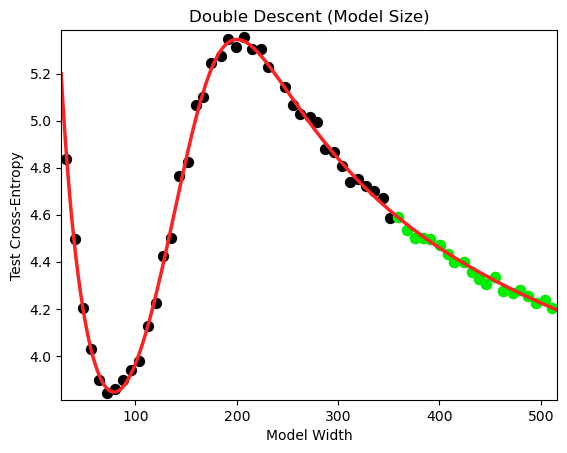
\includegraphics[width=0.48\textwidth]{figures/double_descent/double_descent__model_size.png}
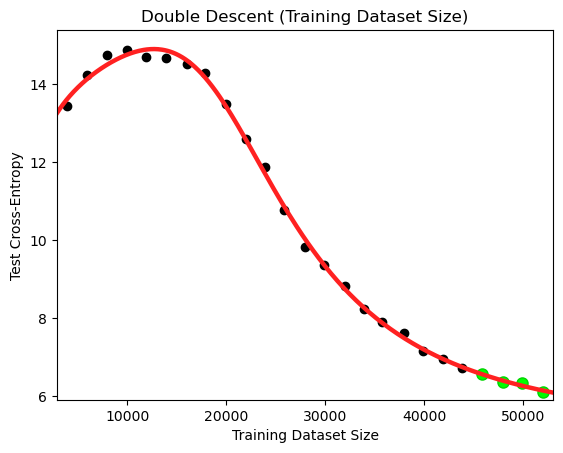
\includegraphics[width=0.48\textwidth]{figures/double_descent/double_descent__dataset_size_1.png}

    \caption{
    Fit of BNSL to Double Descent. Both plots are of transformers trained to do neural machine translation via minimizing cross-entropy. Experimental data of left figure is obtained from Figure 8 top of \cite{nakkiran2021deep}; ``Model Width" on the x-axis refers to embedding dimension $d_{model}$ of the transformer. Experimental data of right figure is obtained from Figure 11b of \cite{nakkiran2021deep}.
    }
    \label{fig:double_descent}
\end{figure*}
\FloatBarrier

\subsection{Inflection Points}
\label{section:Inflection_Points}
We show that BNSL is capable of modeling and extrapolating the scaling behavior of tasks that have an inflection point on a linear-linear plot such as the task of arithmetic (4 digit addition). Other functional forms are mathematically incapable of expressing inflection points on a linear-linear plot (as shown in Section 3) and as a result are mathematically incapable of expressing and modeling inflection points (on a linear-linear plot) that are present in the scaling behaviour of 4 digit addition. In Figure \ref{fig:arithmetic} left, we show that BNSL expresses and accurately models the inflection point present in the scaling behaviour of 4 digit addition and as a result accurately extrapolates the scaling behaviour of 4 digit addition.

\FloatBarrier
\begin{figure*}[htbp]
    \centering


%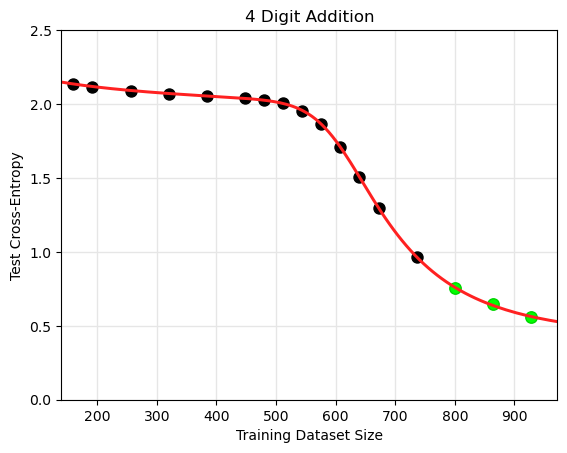
\includegraphics[width=0.48\textwidth]{figures/arithmetic/4_digit_addition__dataset_size.png}
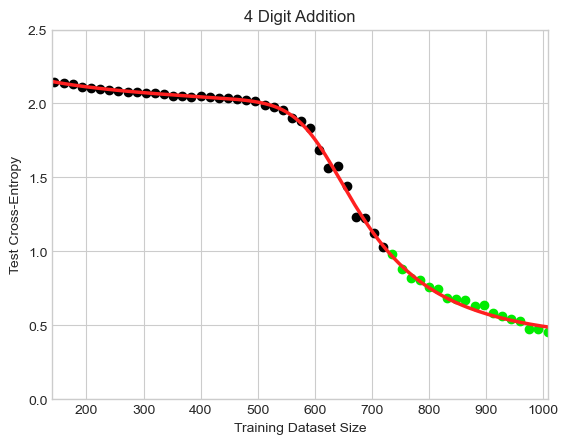
\includegraphics[width=0.48\textwidth]{figures/arithmetic/4_digit_addition__dataset_size__very_first_version.png}
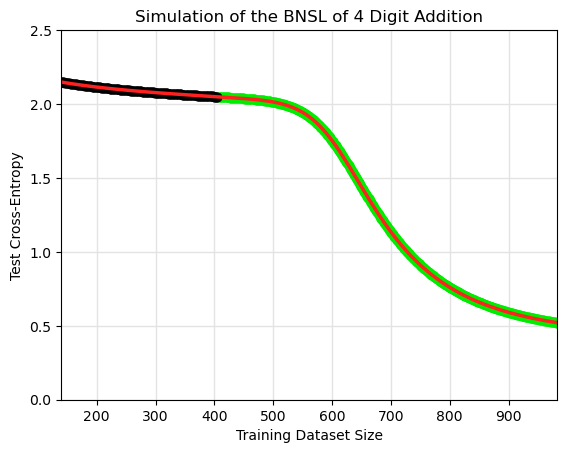
\includegraphics[width=0.48\textwidth]{figures/arithmetic/4_digit_addition__dataset_size__very_first_version__simulation_limit.png}

    \caption{
    4 Digit Addition. Note that these plots are linear-linear. Each point in the left plot is the mean of greater than 100 seeds at that dataset size. In the left plot, each point is gathered from a model trained to do the task of 4 digit addition. In the right plot, each point is gathered from a noiseless simulation of the BNSL of the task of 4 digit addition.
    }
    \label{fig:arithmetic}
\end{figure*}
\FloatBarrier

\subsection{The Limit of the Predictability of Scaling Behavior}
\label{section:limit_of_agi_superforecasting}
We use BNSL to glean insights about the limit of the predictability of scaling behavior. Recent papers \citep{ganguli2022predictability, wei2022emergent} have advertised many task as having ``unpredictable" scaling behavior, the most famous of which being the task of arithmetic. In the previous section and in Figure \ref{fig:arithmetic} left, we successfully predicted (i.e. extrapolated) the scaling behavior of 4 digit addition (arithmetic). However, we are only able to accurately extrapolate the scaling behaviour if given some points from training runs with a training dataset size of at least 720, and the break in which the scaling behaviour of 4 digit addition transitions from one power law to another steeper power law happens at around training dataset size of 415. Ideally, one would like be able to extrapolate the entire scaling behavior by fitting only points from before the break. In Figure \ref{fig:arithmetic} right, we use a noiseless simulation of the BNSL of 4 digit addition to show what would happen if one had infinitely many training runs / seeds to average out all the noisy deviation between runs such that one could recover (i.e. learn via a curve-fitting library such as SciPy \cite{virtanen2020scipy}) the learned constant of the BNSL as well as possible. When using this noiseless simulation, we find that we are only able to accurately extrapolate the scaling behaviour if given some points from training runs with a training dataset size of at least 415, which is very close to the break. This implies that very near to the break there is limit as to how small the supremum of the x-axis of the points used for fitting can be if one wants to perfectly extrapolate the scaling behavior, even if one has infinitely many seeds / training runs.

\subsection{Reinforcement Learning}

TODO: Does RL just go in the appendix because we don't have enough points to get good extrapolations for RL?

\FloatBarrier
\begin{figure*}[htbp]
    \centering


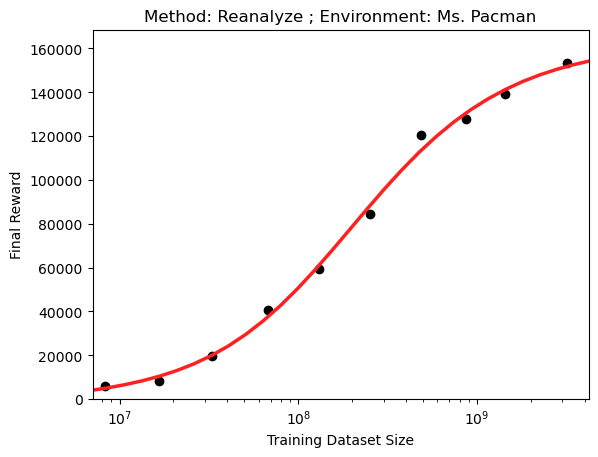
\includegraphics[width=0.48\textwidth]{figures/rl/reanalyze/reanalyze__ms_pacman_dataset_size__fit.png}


    \caption{
    Fit of BNSL to Figure 1 of \cite{schrittwieser2021online}.
    }
    \label{fig:rl_scaling}
\end{figure*}
\FloatBarrier

%\subsection{BIG Bench Emergent}
%Probably will just finish it for rebuttals